\documentclass[xcolor=dvipsnames]{beamer}
\usepackage{ctex}
\usepackage{xypic}
\usepackage{amsfonts,amssymb}
\usepackage{multirow}
\usepackage{fancybox}
\usepackage{nameref}
\usepackage[titletoc]{appendix}

\usepackage{tikz}
\usetikzlibrary{calc,trees,positioning,arrows,chains,shapes.geometric,
decorations.pathreplacing,decorations.pathmorphing,shapes,
matrix,shapes.symbols}
\usepackage[european]{circuitikz}
\usetheme{CambridgeUS}
\usecolortheme[named=Blue]{structure}
\linespread{1.2}
\begin{document}
\normalsize
\title{中断控制器的设计与实现}
\author {王凯祺}


\begin{frame}
\titlepage
\end{frame}

\begin{frame}
	\frametitle{总览}
	
	1. 选题背景
	
	2. 技术路线
	
	3. 设计过程
	
	4. 效果评价
\end{frame}

\begin{frame}
    \frametitle{选题背景}
    
    为什么选择中断控制器,而不选其他?
    
    \pause
    
    我们的课本仅用了 6 页(Section 4.9 Exceptions, Page 314 - 319)简单地介绍了系统中断,并没有把系统中断的过程、原理讲得十分透彻。
    
    我希望自己设计一个中断控制器,填补课本上在系统中断的这块缺失。
	
\end{frame}

\begin{frame}
	\frametitle{技术路线}

	使用 Vivado 作为设计、仿真软件。
	
	使用 Verilog 语言编写源程序。
	
	如何测试中断控制器?
	
	\pause
	
	使用之前实验课设计的多周期 CPU ,配合我设计的中断指令,对中断控制器进行测试。
	
	测试通过后,将中断控制器集成到 CPU ,那么就变成了能处理中断的多周期 CPU 。

\end{frame}

\begin{frame}
	\frametitle{设计过程}
	\framesubtitle{中断处理流程}
	
	\begin{figure}
		\centering
		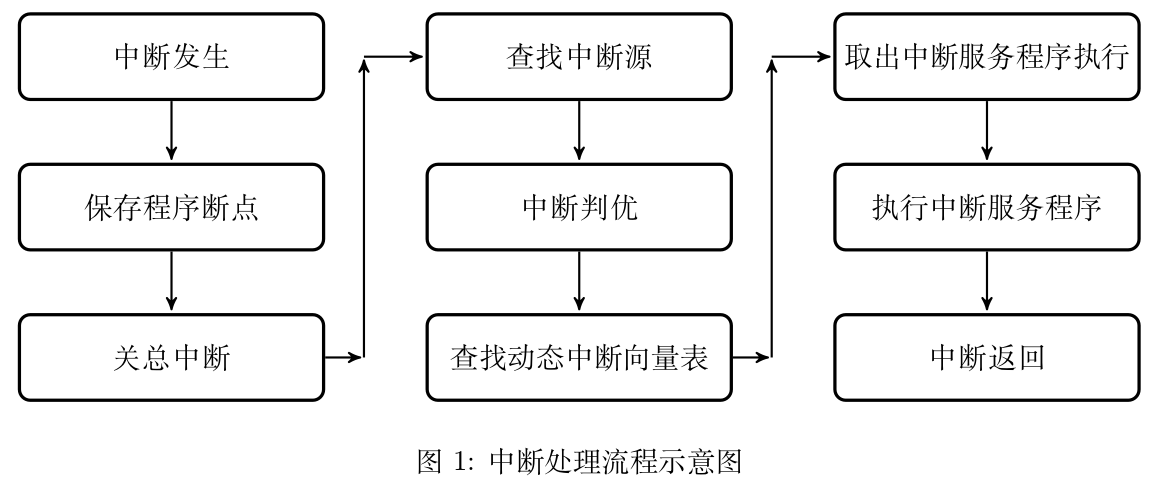
\includegraphics[scale=0.25]{img/1.png}
	\end{figure}
\end{frame}

\begin{frame}
	\frametitle{设计过程}
	\framesubtitle{中断控制器设计}
	
	\begin{figure}
		\centering
		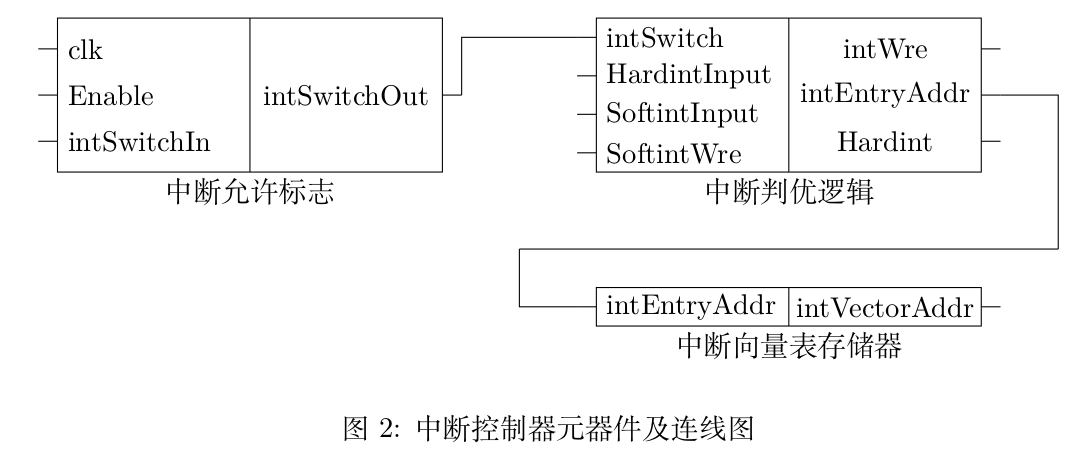
\includegraphics[scale=0.25]{img/2.png}
	\end{figure}
	
	中断控制器是一个中断判优的组合电路,根据输入的中断源,选择优先级最高的响应,并把对应的中断入口地址接到中断向量表存储器中,由中断向量表存储器查询中断向量地址,接到PC输入端。
\end{frame}

\begin{frame}
	\frametitle{设计过程}
	\framesubtitle{中断判优}
	
	\begin{figure}
		\centering
		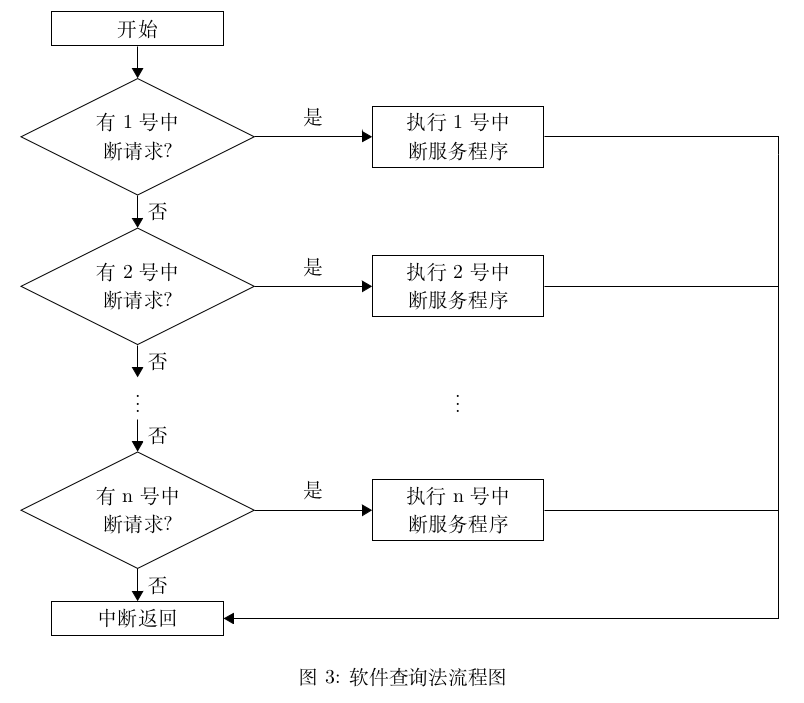
\includegraphics[scale=0.25]{img/3.png}
	\end{figure}
\end{frame}


\begin{frame}
	\frametitle{设计过程}
	\framesubtitle{堆栈设计}	
	
	\begin{figure}
		\centering
		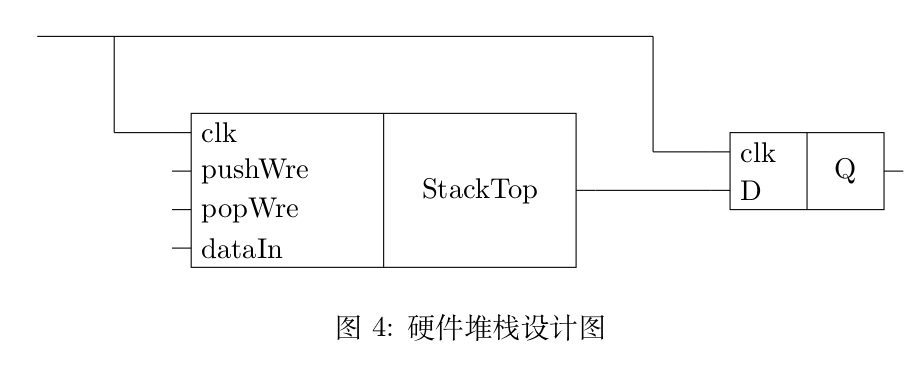
\includegraphics[scale=0.25]{img/4.png}
	\end{figure}
	
	中断服务程序结束后,必须能正确地返回到被中断的断点处继续原来程序的执行。为了保存断点位置,同时为了支持中断嵌套,我们需要实现一个硬件堆栈。
\end{frame}	

\begin{frame}
	\frametitle{设计过程}
	\framesubtitle{重新设计 CPU 状态}
	
	为了测试中断控制器,我们还需要修改多周期 CPU ,使该 CPU 可以处理中断。
	
\end{frame}

\begin{frame}
	\frametitle{设计过程}
	\framesubtitle{重新设计 CPU 状态(不含中断控制器的多周期 CPU 状态转移图)}
	
	\begin{figure}
		\centering
		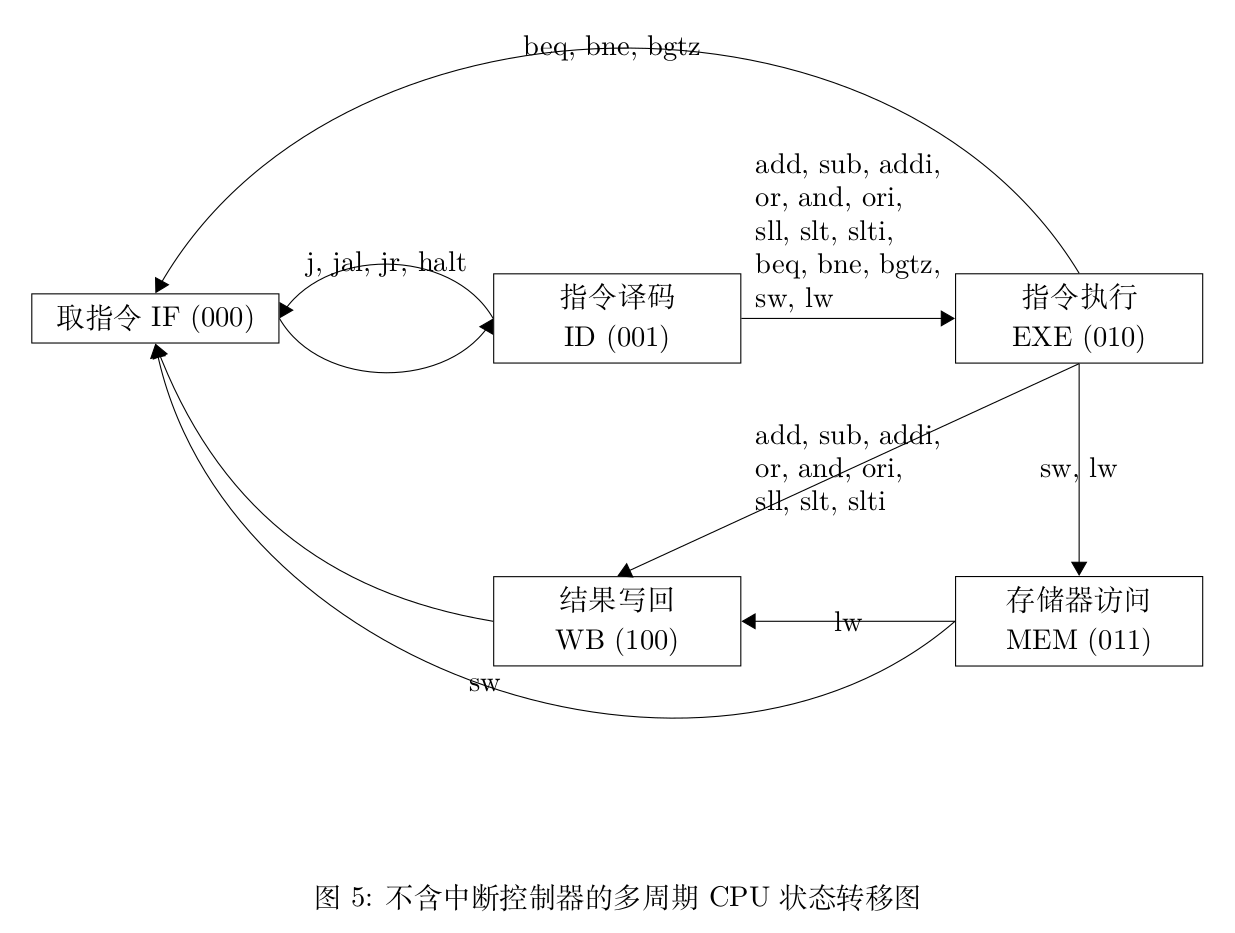
\includegraphics[scale=0.25]{img/5.png}
	\end{figure}
\end{frame}

\begin{frame}
	\frametitle{设计过程}
	\framesubtitle{重新设计 CPU 状态(含中断控制器的多周期 CPU 状态转移图)}
	
	\begin{figure}
		\centering
		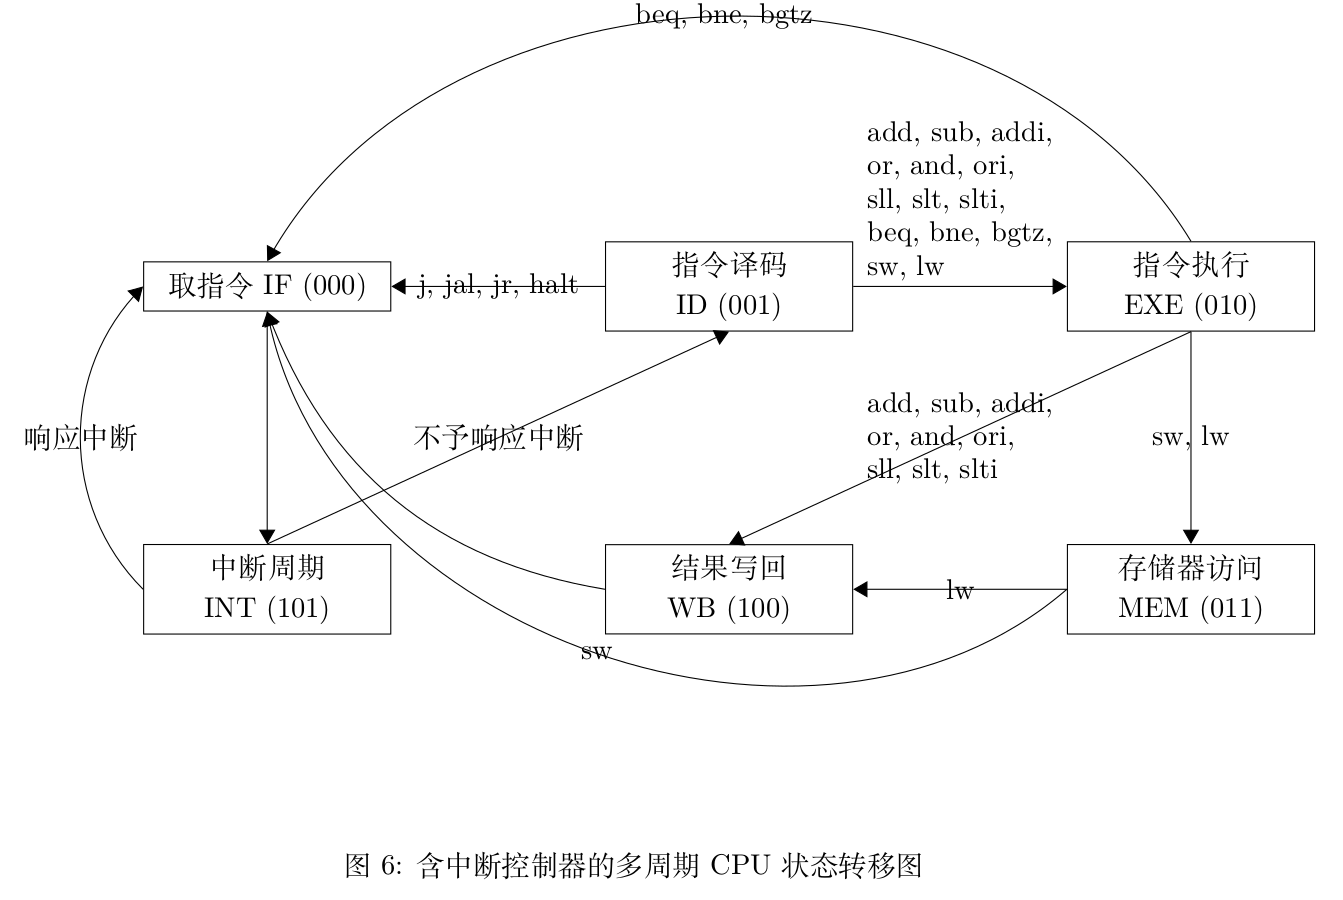
\includegraphics[scale=0.25]{img/6.png}
	\end{figure}
\end{frame}



\begin{frame}
	\frametitle{设计过程}
	\framesubtitle{数据通路}
	
	\begin{figure}
		\centering
		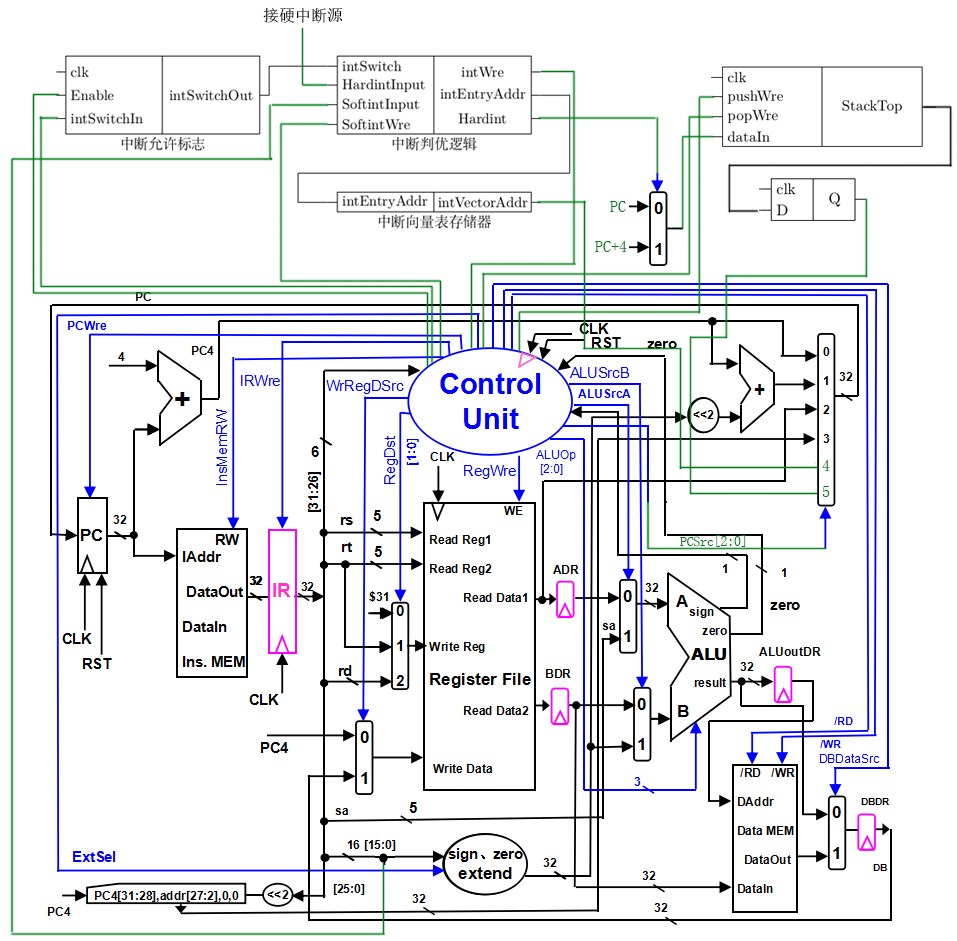
\includegraphics[scale=0.25]{../pics/DataPath.png}
	\end{figure}
\end{frame}

\begin{frame}
	\frametitle{设计过程}
	\framesubtitle{数据通路}
	
	\begin{figure}
		\centering
		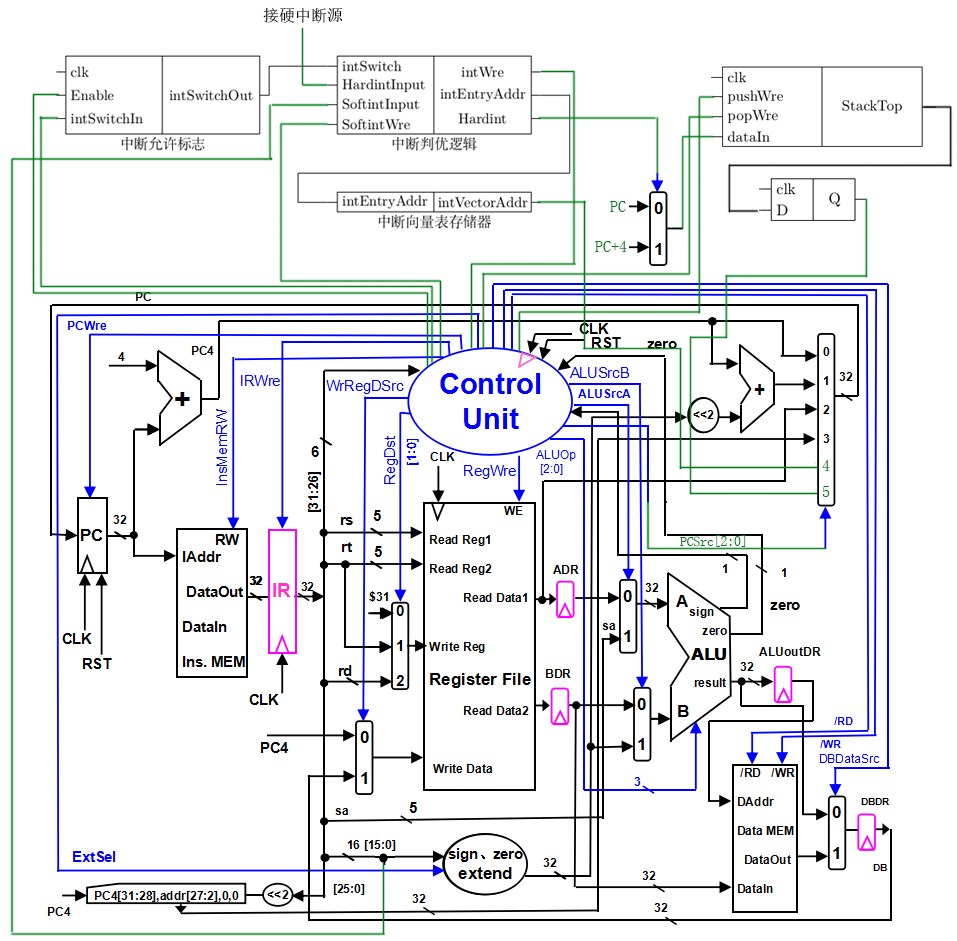
\includegraphics[scale=0.45]{../pics/DataPath.png}
	\end{figure}
\end{frame}

\begin{frame}
	\frametitle{设计过程}
	\framesubtitle{模拟仿真}
	
	\begin{figure}
		\centering
		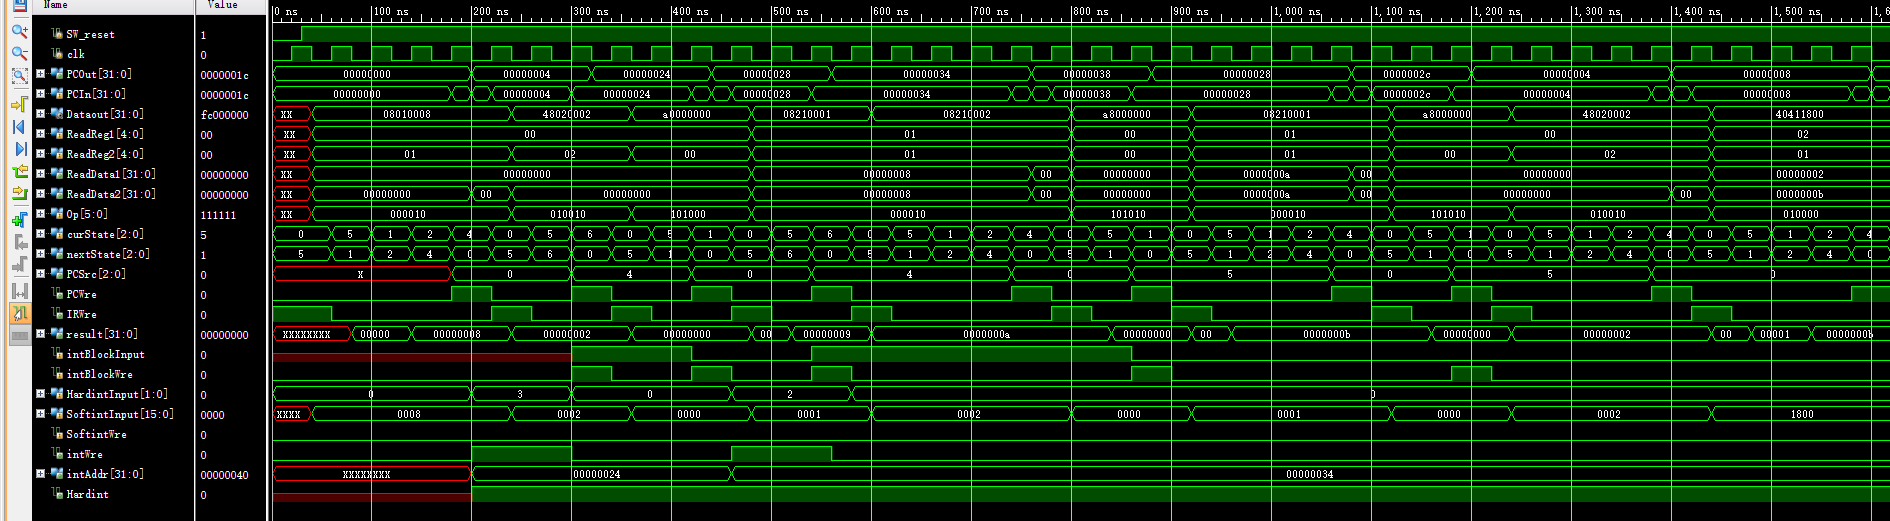
\includegraphics[scale=0.3]{../pics/img_full_1.png}
	\end{figure}
\end{frame}

\begin{frame}
	\frametitle{效果评价}
	自主设计	
	
	能处理软硬中断
	
	能处理中断嵌套
	
	能处理多中断判优
	
	填补了课本上在中断控制方面的空白
	
\end{frame}	

\begin{frame}
	\frametitle{致谢}
	
	感谢李国桢教授提供课堂交流平台!

	感谢何朝东老师提供多周期 CPU 数据通路图!	
	
	感谢同学们的聆听!
	
\end{frame}

\end{document}
